\documentclass[border=8pt]{standalone}
\usepackage{tikz}
\usetikzlibrary{arrows.meta,positioning,calc,fit}
\begin{document}
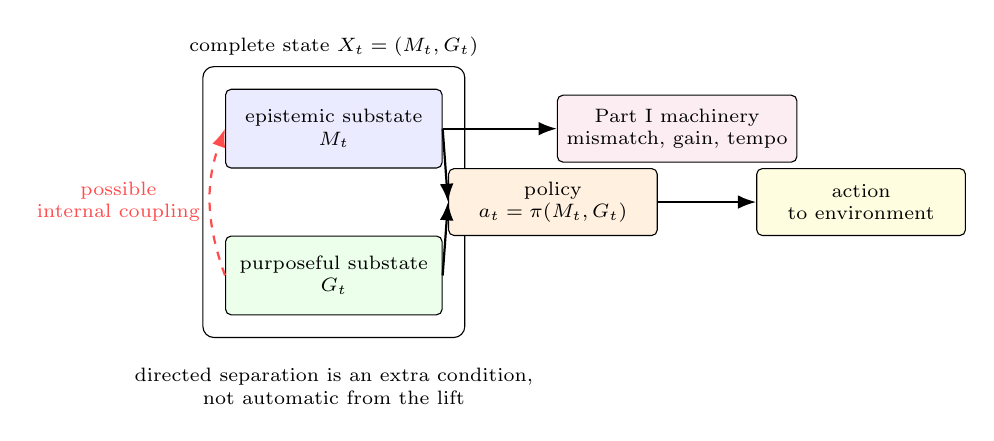
\begin{tikzpicture}[
  box/.style={draw, rounded corners=2pt, align=center, minimum width=2.65cm, minimum height=0.85cm, font=\scriptsize},
  state/.style={draw, rounded corners=2pt, align=center, minimum width=2.75cm, minimum height=1.0cm, font=\scriptsize},
  note/.style={align=center, font=\scriptsize},
  arr/.style={-Latex, thick},
  dasharr/.style={-Latex, thick, dashed}
]

\node[state, fill=blue!8] (m) {epistemic substate\\$M_t$};
\node[state, fill=green!8, below=0.85cm of m] (g) {purposeful substate\\$G_t$};
\node[draw, rounded corners=4pt, fit=(m)(g), inner sep=8pt, label={[font=\scriptsize]above:complete state $X_t=(M_t,G_t)$}] (x) {};

\node[box, fill=purple!7, right=1.45cm of m] (parti) {Part I machinery\\mismatch, gain, tempo};
\node[box, fill=orange!12, right=1.45cm of $(m)!0.5!(g)$] (policy) {policy\\$a_t=\pi(M_t,G_t)$};
\node[box, fill=yellow!12, right=1.25cm of policy] (act) {action\\to environment};

\draw[arr] (m) -- (parti);
\draw[arr] (m.east) -- (policy.west);
\draw[arr] (g.east) -- (policy.west);
\draw[arr] (policy) -- (act);

\draw[dasharr, red!70] (g.west) to[bend left=20] node[left, font=\scriptsize, align=center] {possible\\internal coupling} (m.west);
\node[note, below=0.55cm of g] {directed separation is an extra condition,\\not automatic from the lift};

\end{tikzpicture}
\end{document}
